\themeG
\chapter{Hauteurs et médiatrices du triangle}
\label{S26}

\textcolor{red}{\bf Connaissances :}
   \begin{connaissances}
      \item Triangle : hauteurs et médiatrices.
   \end{connaissances}

\vfill

\begin{debat}{Débat : mot valise}
   Un {\bf mot-valise} est un mot formé par l'accolement du début d'un mot et la fin d'un autre mot. À l'heure actuelle, on invente régulièrement des mots-valises : {\it Brexit} pour Britain et exit, {\it Twictée} pour Twitter et dictée, {\it pourriel} pour poubelle et courriel\dots \par
      Les maths n'échappent par à la règle et le mot {\it médiatrice} est un mot-valise qui vient de médiane (dans un triangle, droite joignant un sommet au milieu du côté opposé) et bissectrice (droite coupant un angle en deux angles égaux). Il a été formé en 1923, donc très récemment.
   \tcblower
      \begin{pspicture}(0,0)(3,2.5)
         \psline[linearc=0.2,linewidth=2mm,linecolor=Black!70](1,2)(1,2.4)(2,2.4)(2,2)
         \psframe[fillstyle=solid,fillcolor=DarkGrey,framearc=0.3](0,0)(3,2)
         \psframe[fillstyle=solid,fillcolor=Brown](0.55,0)(0.85,2)
         \psarc(0.7,0.8){0.15}{180}{360}
         \psdot(0.7,0.85)
         \psframe[fillstyle=solid,fillcolor=Brown](2.45,0)(2.15,2)
         \psarc(2.3,0.9){0.15}{180}{360}
         \psdot(2.3,0.95)
         \psset{linecolor=Black!50,linewidth=1.5mm}
         \psarc(0,0){0.3}{2}{88}
         \psarc(3,0){0.3}{92}{178}
         \psarc(3,2){0.3}{182}{268}
         \psarc(0,2){0.3}{272}{358}
      \end{pspicture}
\end{debat}

\hfill {\gray Vidéo : \href{https://www.youtube.com/watch?v=M7npDrRJm6E}{\bf Les mots-valises}, chaîne YouTube {\it Image et communication}, épisode d'{\it Au pied de la lettre}.}


%%% Approche %%%
\begin{Maquette}[Cours]{Theme={Activité d'approche},Couleur={SteelBlue}}

   \AAtitre{Des droites concourantes}

      {\it Objectifs : tracer les médiatrices d'un triangle ; démontrer que les médiatrices d'un triangle sont concourantes.}

      \begin{AActivite}

         \AApartie{Construction de médiatrices}
            \begin{enumerate}
               \item Expliquer à l'oral la construction de la médiatrice d'un segment d'après les schémas suivants : 
                  \begin{center}
                     {\psset{unit=0.75}
                     \begin{pspicture}(0,0)(5,3.5)
                        \pstGeonode[PosAngle=180,linecolor=DodgerBlue](1,3){M}
                        \pstGeonode[PointSymbol=none,PointName=none](0,0){E}(4,3){F}
                        \pstOrtSym[linecolor=DodgerBlue]{E}{F}{M}[N] 
                     \end{pspicture}
                     \begin{pspicture}(0,-0.25)(5,3.5)
                        \pstGeonode[PosAngle=180,linecolor=DodgerBlue](1,3){M}
                        \pstGeonode[PointSymbol=none,PointName=none](0,0){E}(4,3){F}
                        \psarc[linecolor=DodgerBlue,linestyle=dashed](1,3){2}{260}{300}
                        \psarc[linecolor=DodgerBlue,linestyle=dashed](1,3){2}{320}{360}
                        \pstOrtSym[linecolor=DodgerBlue]{E}{F}{M}[N]  
                        \psarc[linecolor=DodgerBlue,linestyle=dashed](3.18,0.16){2}{80}{120}
                        \psarc[linecolor=DodgerBlue,linestyle=dashed](3.18,0.16){2}{140}{175}
                     \end{pspicture} 
                     \begin{pspicture}(0,-0.25)(4,3.5)
                        \pstGeonode[PosAngle=180,linecolor=DodgerBlue](1,3){M}
                        \pstGeonode[PointSymbol=none,PointName=none](0,0){E}(4,3){F}
                        \psarc[linecolor=DodgerBlue,linestyle=dashed](1,3){2}{260}{300}
                        \psarc[linecolor=DodgerBlue,linestyle=dashed](1,3){2}{320}{360}
                        \pstOrtSym[linecolor=DodgerBlue]{E}{F}{M}[N]  
                        \psarc[linecolor=DodgerBlue,linestyle=dashed](3.18,0.16){2}{80}{120}
                        \psarc[linecolor=DodgerBlue,linestyle=dashed](3.18,0.16){2}{140}{175} 
                        \pstMediatorAB[CodeFig=true,PointName=none,PointSymbol=none]{M}{N}{I}{F}  
                        \pstMediatorAB[PointName=none,PointSymbol=none]{N}{M}{I}{E}     
                        \pstLineAB[linecolor=Crimson,linewidth=0.05]{E}{F} 
                     \end{pspicture}}
                  \end{center}
               \item Donner une définition de la médiatrice d'un segment : \par \smallskip
                  \pointilles
               \item Donner une propriété de la médiatrice d'un segment : \par \smallskip
                  \pointilles
               \item Tracer la médiatrice de tous les côtés de ces deux polygones.
                  \begin{center}
                     {\psset{unit=0.8}
                     \begin{pspicture}(0.5,-0.5)(20,5)
                        \pspolygon(0,2)(6,0)(9,3)
                        \pspolygon(12,0)(20,1)(16,5)(12,3)
                     \end{pspicture}}
                  \end{center}
               \item Pour quel polygone les médiatrices sont-elles concourantes ? \pointilles
            \end{enumerate}

      \AApartie{Démonstration}
         \begin{enumerate}
            \setcounter{enumi}{5}
            \item Sur une feuille, tracer un triangle $ABC$ puis tracer la médiatrice de $[AB]$ et la médiatrice de $[BC]$. \par
               Placer $O$, point d'intersection de ces deux médiatrices.
            \item $O$ se situe sur la médiatrice de $[AB]$. Comparer les longueurs $OA$ et $OB$ : \pointilles \smallskip
            \item $O$ se situe sur la médiatrice de $[BC]$. Comparer les longueurs $OB$ et $OC$ : \pointilles \smallskip
            \item En déduire une relation entre $OA$ et $OC$ : \pointilles \smallskip
            \item Que peut-on dire du point $O$ par rapport à $[CA]$ ? \pointilles \smallskip
            \item Tracer le cercle de centre $O$ passant par $A$. Que remarque-t-on ? \pointilles \smallskip
            \item Conclure : \pointilles
         \end{enumerate}

      \end{AActivite}

\end{Maquette}


%%%Trace écrite %%%
\begin{Maquette}[Cours]{Theme={Trace écrite},Couleur={0.4[SteelBlue,Black]}}

   %%%1
   \section{Médiatrices d'un triangle}

      \begin{definition*}{}
         Les \textbf{médiatrices} d'un triangle sont les médiatrices des côtés du triangle, c'est-à-dire les trois droites perpendiculaires aux côtés qui passent par leur milieu.
      \end{definition*}

      Pour tracer la médiatrice du segment $[AB]$ au compas, on choisit un écartement au compas et on trace deux arcs de cercle à partir de $A$ et de $B$ de part et d'autre du segment [$AB]$. Puis on trace la droite passant par les deux points formés par l'intersection des arcs de cercle. \bigskip

      \begin{tabular}{C{4}C{7.2}C{5.4}}
         \raisebox{-3cm}{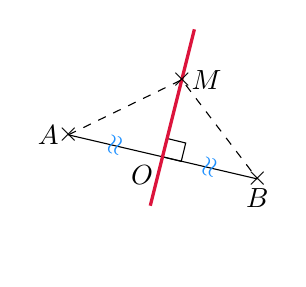
\begin{tikzpicture}[scale=0.8]
            \draw (0.5,2.825)--(3.5,2.125);
            \draw[shift={(2,2.475)}, rotate=-13.7] (0,0) rectangle (0.3,0.3);
            \draw[very thick, color=Crimson] (1.8,1.7)--(2.5,4.5);
            \foreach \x/\y/\N/\pos in {0.5/2.825/A/left, 3.5/2.125/B/below, 2.3/3.7/M/right} {\draw (\x,\y) node{$\times$};\draw (\x,\y) node[\pos]{$\N$}; } 
            \draw (2,2.5) node[below left] {$O$};
            \draw (1.25,2.65) node[color=DodgerBlue, rotate=76] {$\approx$};
            \draw (2.75,2.3) node[color=DodgerBlue, rotate=76] {$\approx$};
            \draw[dashed] (0.5,2.825)--(2.3,3.7)--(3.5,2.125);
            \draw (0,1) node {};
         \end{tikzpicture}}
         &
         \begin{propriete*}{}
            Si un point appartient à la médiatrice d'un segment, alors il est équidistant des extrémités de ce segment.
         \end{propriete*}
         &
         \raisebox{-1cm}{\parbox{5cm}{Ici, $M$ appartient à la médiatrice de $[AB]$. \par Donc $MA=MB$.}} \\
         & & \\
         {\psset{unit=0.5,linewidth=0.03}
         \begin{pspicture}(-1,-2)(6,3.5)
            \psset{CodeFig=true,PointSymbol=none,linecolor=Crimson}
            \pstTriangle{A}(5,0){B}(1.5,3){C}
            \pstCircleABC[RightAngleSize=0.2,CodeFigColor=black]{A}{B}{C}{O}
         \end{pspicture}}
         &
         \begin{propriete*}{}
            Dans un triangle, les trois médiatrices sont concourantes en un point qui est le centre du cercle circonscrit au triangle.
         \end{propriete*}
         &
         \raisebox{-1cm}{\parbox{5cm}{Ici, les médiatrices à $[AB]$, $[BC]$ et $[CA]$ se coupent en $O$ qui est le centre du cercle passant par les trois sommets $A$, $B$ et $C$.}} \\
      \end{tabular}
   

   %%%2
   \section{Hauteurs d'un triangle}

      \begin{definition*}{}
         Les \textbf{hauteurs} d'un triangle sont les hauteurs relatives aux sommets du triangle, c'est-à-dire les trois droites perpendiculaires aux côtés qui passent par le sommet opposé.
      \end{definition*}

      Pour tracer la hauteur dans un triangle issue d'un sommet, on trace la droite passant par ce sommet et perpendiculaire au côté opposé. \bigskip

      \begin{tabular}{C{4}C{6.9}C{5.6}}
         {\psset{unit=0.7,linewidth=0.03}
         \begin{pspicture}(-1,-0.8)(4.5,3.5)
            \psset{CodeFig=true, PointSymbol=none,RightAngleSize=0.2}
            \pstTriangle{A}(4,0){B}(1.5,2.5){C}
            \pstProjection[PointName=none,CodeFigColor=Crimson]{B}{A}{C}
            \pstProjection[PointName=none,CodeFigColor=Crimson]{A}{C}{B}
            \pstProjection[PointName=none,CodeFigColor=black]{C}{B}{A}
            \rput(1.8,0.9){$H$}
         \end{pspicture}}
         &
         \begin{propriete*}{}
            Dans un triangle, les trois hauteurs sont concourantes en un point appelé orthocentre du triangle.
         \end{propriete*}
         &
         \raisebox{-1cm}{\parbox{5.6cm}{Ici, $H$ est le point de concours de la hauteur issue de $C$ et de celle issue de $B$. \par Donc, $[AH]$ est la hauteur issue de $A$.}} \\
      \end{tabular}

\end{Maquette}


%%% Exercices %%%
\begin{Maquette}[Fiche,CorrigeFin,Colonnes=2]{}
   
   \begin{multicols}{2}

      \begin{exercice} %1
         Suivre le programme suivant en codant les éléments construits :
         \begin{enumerate}
            \item Construire un triangle $CJR$ quelconque.
            \item Tracer en rouge la médiatrice du segment $[JR]$ à l'aide du compas et d'une règle graduée.
            \item Tracer en noir la médiatrice du segment $[CJ]$ à la règle graduée et à l'équerre.
            \item Construire la médiatrice $(d)$ du segment $[CR]$ avec seulement une équerre (non graduée).
         \end{enumerate}
      \end{exercice}    
      
      \begin{Solution}
         \begin{pspicture}(-0.5,1)(6,4.25)
            \pstGeonode[CurveType=polygon,PosAngle={200,0,90}](1,1){C}(5.5,1){J}(2.5,4){R}
            \psset{CodeFig=true,CodeFigColor=black,PointName=none,linestyle=dashed}
            \pstMediatorAB[linecolor=Crimson,SegmentSymbol=pstslash]{J}{R}{I}{K}
            \pstMediatorAB[linecolor=black,SegmentSymbol=pstslashh]{C}{J}{L}{M}
            \pstMediatorAB[linecolor=RoyalBlue,SegmentSymbol=pstslashhh]{R}{C}{N}{d}     
            \rput(2.2,2.3){\cor{$(d)$}}
         \end{pspicture}
      \end{Solution}    

      
      \begin{exercice} %2
         Dans chaque cas, construire le triangle puis son cercle circonscrit de centre $O$.
         \begin{enumerate}
            \item Triangle $SKI$ tel que : \par
               $SI = \Lg{8} \; ; \widehat{KSI} =\ang{65}$et $\widehat{KIS} =\ang{45}$.
            \item Triangle $GYM$ tel que : \par
               $GM = \Lg{4} \; ; GY = \Lg{5}$ et $\widehat{YGM} =\ang{103}$.
            \item Triangle $TIR$ tel que : \par
               $TIR$ est isocèle en $T$ ; $TI =\Lg{8}$ et $IR =\Lg{5,5}$.
            \item Triangle $VTC$ tel que : \par
               $VTC$ est un triangle équilatéral de côté \Lg{4}.
         \end{enumerate}
      \end{exercice}
      
      \begin{Solution}
         \begin{pspicture}(0,-3)(9,5.75)
            \pstTriangle(0,0){S}(8,0){I}(2.34,5.66){K}
            \pstCircleABC[CodeFig=true,CodeFigColor=RoyalBlue,SegmentSymbolA=pstslash,SegmentSymbolB=pstslashh,SegmentSymbolC=pstslashhh]{S}{K}{I}{O}
            \pstLabelAB[offset=-3mm]{S}{I}{\Lg{8}}
            \pstMarkAngle{I}{S}{K}{\ang{65}}
            \pstMarkAngle[MarkAngleType=double]{K}{I}{S}{\ang{45}}
         \end{pspicture}
       
         \begin{pspicture}(-2,-1)(6,6)
            \pstTriangle(0,0){G}(4,0){M}(-1.12,4.87){Y}
            \pstCircleABC[CodeFig=true,CodeFigColor=RoyalBlue,SegmentSymbolA=pstslash,SegmentSymbolB=pstslashh,SegmentSymbolC=pstslashhh]{G}{M}{Y}{O}
            \pstLineAB{G}{M}
            \pstLineAB{G}{Y}
            \pstLineAB{Y}{M}
            \pstLabelAB[offset=-3mm]{G}{M}{\Lg{4}}
            \pstLabelAB[offset=-3mm]{Y}{G}{\Lg{5}}
            \pstMarkAngle{Y}{M}{G}{\ang{45}}
            \pstMarkAngle{M}{G}{Y}{\ang{103}}
         \end{pspicture}
      
         \begin{pspicture}(0,-3)(8,7)
            \pstTriangle(0,0){T}(8,0){I}(6.11,5.16){R}
            \pstCircleABC[CodeFig=true,CodeFigColor=RoyalBlue,SegmentSymbolA=pstslash,SegmentSymbolB=pstslashh,SegmentSymbolC=pstslashh]{T}{R}{I}{O}
            \pstLineAB{T}{R}
            \pstLineAB{T}{I}
            \pstLineAB{I}{R}
            \pstLabelAB[offset=-3mm]{T}{I}{\Lg{8}}
            \pstLabelAB{R}{I}{\Lg{5,5}}
         \end{pspicture}
         
         \begin{pspicture}(-2.5,-2)(5,4.5)
            \pstTriangle(0,0){V}(4,0){T}(2,3.46){C}
            \pstCircleABC[CodeFig=true,CodeFigColor=RoyalBlue,SegmentSymbolA=pstslashh,SegmentSymbolB=pstslashh,SegmentSymbolC=pstslashh]{V}{C}{T}{O}
            \pstLineAB{V}{C}
            \pstLineAB{V}{T}
            \pstLineAB{T}{C}
            \pstLabelAB[offset=-3mm]{V}{T}{\Lg{4}}
         \end{pspicture}
      \end{Solution}
      

      \begin{exercice} %3
         Construction de hauteurs.
         \begin{enumerate}
            \item Construire un triangle $BLE$ puis tracer :
            \begin{itemize}
               \item en bleu, la hauteur issue du sommet $E$ ;
               \item en noir, la hauteur issue du sommet $B$ ;
               \item en rouge, la hauteur relative à $[BE]$.
            \end{itemize}
             \item Quelle remarque peut-on faire ?
         \end{enumerate} 
      \end{exercice}
      
      \begin{Solution}
         \begin{pspicture}(-1,0)(6,6)
            \pstGeonode[CurveType=polygon,PosAngle={200,0,90}](0,1){B}(6,2){L}(4,5){E}
            \pstProjection[CodeFig=true,CodeFigColor=RoyalBlue,PointName=none]{B}{L}{E}
            \pstProjection[CodeFig=true,CodeFigColor=black,PointName=none]{L}{E}{B}
            \pstProjection[CodeFig=true,CodeFigColor=Crimson,PointName=none]{E}{B}{L}
         \end{pspicture} \par
         On remarque que \cor{les hauteurs sont concourantes} en un point appelé l'orthocentre du triangle.
      \end{Solution}
      
      
      \begin{exercice} %4
         Tracer les hauteurs dans les cas suivants :
         \begin{enumerate}
            \item Un triangle $ONE$ ayant trois angles aigus, quelle remarque peut-on faire sur l'orthocentre ?
            \item Un triangle $TWO$ tel que l'angle $\widehat{TWO}$ soit obtus, quelle remarque peut-on faire sur l'orthocentre ?
            \item Un triangle $TRE$ rectangle en $R$, quelle remarque peut-on faire sur l'orthocentre ?
         \end{enumerate}
      \end{exercice}
      
      \begin{Solution}
         \begin{pspicture}(-1,-0.5)(6,5)
            \pstGeonode[CurveType=polygon,PosAngle={200,0,90}](0,1){O}(5,0.5){N}(2,4){E}
            \psset{CodeFig=true,CodeFigColor=Crimson,PointName=none}
            \pstProjection{N}{O}{E}
            \pstProjection{O}{E}{N}
            \pstProjection{E}{N}{O}
            \rput(5,3.5){\parbox{2.5cm}{L'orthocentre se situe \cor{à l'intérieur du triangle}}}
         \end{pspicture}
         
         \begin{pspicture}(0,-2.2)(8,4)
            \pstGeonode[CurveType=polygon,PosAngle={200,0,90}](1,3){T}(5.5,1){W}(8,3.5){O}
            \psset{CodeFig=true,CodeFigColor=Crimson,PointName=none,linecolor=Crimson,linestyle=dashed}
            \pstProjection{T}{W}{O}[A]
            \pstProjection{O}{T}{W}[B]
            \pstProjection{W}{O}{T}[C]
            \pstLineAB[nodesepB=-2.5]{O}{A}
            \pstLineAB[nodesepB=-3]{B}{W}
            \pstLineAB[nodesepB=-2.5]{T}{C}
            \psset{linecolor=black}
            \pstLineAB{W}{C}
            \pstLineAB{W}{A}
            \rput(2,-0.5){\parbox{2.5cm}{L'orthocentre se situe \cor{à l'extérieur du triangle}}}
         \end{pspicture}
         
         \begin{pspicture}(-1,-0.5)(6.5,4.5)
            \pstGeonode[CurveType=polygon,PosAngle={200,0,90}]{T}(6,0){R}(6,3.5){E}
            \psset{CodeFig=true,CodeFigColor=Crimson,PointName=none}
            \psframe(6,0)(5.6,0.4)
            \pstProjection{E}{T}{R}
            \pstLineAB[linestyle=dashed,linecolor=Crimson]{T}{E}
            \rput(1,2.5){\parbox{3cm}{L'orthocentre est \cor{au point $R$} où le triangle est rectangle}}
         \end{pspicture}
      \end{Solution}
      
      
      \begin{exercice} %5
         \begin{enumerate}
         \item Tracer un triangle $YES$ quelconque.
            \item Placer :
            \begin{itemize}
               \item le milieu $O$ du côté $[ES]$ ;
               \item le milieu $U$ du côté $[YS]$ ;
               \item le milieu $I$ du côté $[YE]$.
            \end{itemize}
            \item Tracer le triangle $OUI$ puis ses hauteurs.
            \item Placer le point $T$ orthocentre du triangle $OUI$.
            \item Trace le cercle de centre $T$ et de rayon $[TY]$.
            \item Quelle conjecture peut-on écrire ?
         \end{enumerate}
      \end{exercice}
      
      \begin{Solution}
         \begin{pspicture}(-1,-2)(6,4.5)
            \psset{CodeFig=true}
            \pstGeonode[CurveType=polygon,PosAngle={200,0,90}](0,0){Y}(6,0.5){E}(3.8,4){S}
            \pstMiddleAB[PosAngle=-90,SegmentSymbol=pstslashhh]{Y}{E}{I}
            \pstMiddleAB[SegmentSymbol=pstslash]{Y}{S}{U}
            \pstMiddleAB[PosAngle=30,SegmentSymbol=pstslashh]{E}{S}{O}
            \pstLineAB{O}{U}
            \pstLineAB{O}{I}
            \pstLineAB{I}{U}
            \psset{CodeFigColor=Crimson,PointName=none}
            \pstProjection{O}{U}{I}[J]
            \pstProjection{I}{O}{U}[K]
            \pstProjection{U}{I}{O}
            \pstInterLL[PointName=T,PosAngle=65]{I}{J}{K}{U}{T}
            \pstCircleOA{T}{Y}
         \end{pspicture} \par
         On peut conjecturer que \cor{le centre du cercle circonscrit au triangle $YES$ est l'orthocentre du triangle $OUI$}.
      \end{Solution}
      
      
      \begin{exercice}[Dur] %6
         \begin{enumerate}
            \item Tracer un triangle $BAC$ rectangle en $A$.
            \item Placer un point $M$ à l'extérieur du triangle $ABC$.
            \item La droite perpendiculaire à $(AB)$ passant par $M$ coupe $[AB]$ en $I$ et la droite perpendiculaire à $[AC]$ passant par $M$ coupe $[AC]$ en $J$.
            \item Placer le point $P$ sur la demi-droite $[MI)$ tel que $I$ soit le milieu de $[MP]$ et le point $Q$ sur la demi-droite $[MJ)$ tel que $J$ soit le milieu de $[MQ]$.
            \item Que représente le point $A$ pour le triangle $MQP$ ? Justifier.
         \end{enumerate}
      \end{exercice}
      
      \begin{Solution}
         \begin{pspicture}(0.5,-3.5)(8.5,4)
            \pstGeonode[CurveType=polygon,PosAngle={200,0,90}](1,0){B}(5,0){A}(5,3){C}
            \pstRightAngle{B}{A}{C}
            \pstGeonode[PosAngle={135,-135,45}](2,1.6){M}(2,-1.6){P}(8,1.6){Q}
            \psset{CodeFig=true,CodeFigColor=RoyalBlue}
            \pstProjection[PosAngle=45]{A}{B}{M}[I]
            \pstProjection[PosAngle=45]{A}{C}{M}[J]
            \pstCircleOA{A}{M}
            \psset{linecolor=RoyalBlue}
            \pstSegmentMark[SegmentSymbol=pstslash]{M}{I}
            \pstSegmentMark[SegmentSymbol=pstslash]{P}{I}
            \pstSegmentMark[SegmentSymbol=pstslashh]{M}{J}
            \pstSegmentMark[SegmentSymbol=pstslashh]{Q}{J}
            \pstLineAB{P}{Q}
            \rput(5.5,-1.5){\parbox{4cm}{$A$ est le \cor{centre du cercle circonscrit au triangle $MPQ$}.}}     
         \end{pspicture} \par
         \begin{itemize}
            \item la droite $(CJ)$ est perpendiculaire à la droite $(MQ)$ et coupe le segment $[MQ]$ en son milieu $J$ , il s'agit donc de la médiatrice du segment $[MQ]$ ;
            \item la droite $(BA)$ est perpendiculaire à la droite $(MP)$ et coupe le segment $[MP]$ en son milieu $I$, il s'agit donc de la médiatrice du segment $[MP]$ ;
            \item or, les médiatrices du triangle $MPQ$ sont concourantes en un point qui est le centre de son cercle circonscrit ;
            \item $(CJ)$ et $(BI)$ se coupent en $A$, qui est bien le centre du triangle circonscrit au triangle $MPQ$.
         \end{itemize}
      \end{Solution}
      
      
      \begin{exercice}[Dur] %7
         Lorette avait tracé un triangle $AVU$ au crayon et les médiatrices de deux des côtés au stylo. Son voisin Bilel a effacé le triangle mais a laissé le point $A$ et les deux médiatrices. Reconstruire le triangle de Rose.
         \begin{center}
            \begin{pspicture}(0,0)(6,5.5)
               \rput(1,3.3){$A$}
               \rput(1,3){$\times$}
               \psline(0,0.5)(6,4)
               \psline(4,0)(2.5,4)
            \end{pspicture}
         \end{center}
      \end{exercice}
      
      \begin{Solution}
         Il suffit de construire les points $U$ et $V$ symétriques du point $A$ par rapport aux deux droites déjà tracées.
         \begin{center}
            \begin{pspicture}(0,0)(6,5)
               \pstGeonode[PosAngle=135](1,3){A}
               \pstGeonode[PointName=none,PointSymbol=none](0,0.5){B}(6,4){C}(4,0){D}(2.5,4){E}
               \rput(1,3){$\times$}
               \pstLineAB{B}{C}
               \pstLineAB{E}{D}
               \psset{CodeFig=true,linecolor=RoyalBlue,CodeFigColor=RoyalBlue}
               \pstOrtSym[SegmentSymbol=pstslash]{B}{C}{A}[V]
               \pstOrtSym[SegmentSymbol=pstslashh]{D}{E}{A}[U]
               \pstLineAB{A}{V}
               \pstLineAB{A}{U}
               \pstLineAB{U}{V}
            \end{pspicture}
         \end{center}
      \end{Solution}

   \end{multicols}

\end{Maquette}


%%% Récré %%%
\begin{Maquette}[Cours]{Theme={Activité récréative},Couleur={IndianRed}}
    
   \ARtitre{La droite d'Euler}

      Ouvrir Geogebra et choisir l'onglet \textbf{Géométrie}.

      \ARpartie{Construction de la figure}
         {\hautab{1.3}
         \begin{tabular}{|cp{5.5cm}|p{4.5cm}|p{5cm}|}
            \hline
            & Instructions & Outil GeoGebra & Action \\
            \hline
            {\bf 1.} & \multicolumn{3}{l|}{Construction du {\bf triangle} $ABC$} \\
            & Tracer un triangle $ABC$ & polygone & cliquer en trois points quelconques du plan \\
            \hline
            {\bf 2.} & \multicolumn{3}{l|}{Construction des trois {\bf hauteurs} et de l'orthocentre $H$} \\
            & Tracer les hauteurs du triangle & droites perpendiculaires & sélectionner pour chaque hauteur le sommet et son côté opposé \\
            & Placer l'orthocentre & intersection entre deux objets & sélectionner deux hauteurs parmi les trois \\ 
            & Renommer l'orthocentre en $H$ & clic droit propriétés & nom du point : $H$ \\
            & Effacer les hauteurs & clic droit & décocher \og afficher l'objet \fg \\
            \hline
            {\bf 3.} & \multicolumn{3}{l|}{Construction des trois {\bf médiatrices} et du centre du cercle circonscrit $O$} \\
            & Tracer les médiatrices du triangle & médiatrices & choisir pour chaque médiatrice deux sommets du triangle \\
            & Placer le centre du cercle circonscrit & \dots & \dots \\ 
            & Renommer le centre en $O$ & \dots & \dots \\
            & Tracer le cercle circonscrit & cercle (centre-point) & choisir le centre $O$ et le sommet $A$ \\
            & Effacer les médiatrices & \dots & \dots \\
            \hline
            {\bf 4.} & \multicolumn{3}{p{15cm}|}{Construction des trois {\bf médianes} et du centre de gravité $G$. \newline
            {\it La médiane d'un côté du triangle est la droite passant par le milieu du côté et le sommet opposé. \newline
            Le point de concours des médianes s'appelle le centre de gravité.}} \\
            & Tracer les médianes du triangle  &  milieu ou centre & pour chaque médiane, sélectionner deux sommets du triangle \\
            & & droite passant par deux points & sélectionner un sommet et le milieu du côté opposé \\
            & Placer le centre de gravité & \dots & \dots \\
            & Renommer le centre en G & \dots & \dots \\
            & Effacer les médianes et les milieux & \dots & \dots \\
            \hline
         \end{tabular}}
      
      \ARpartie{Constatations}
         \begin{enumerate}
            \setcounter{enumi}{4}
            \item $H$, $O$ et $G$ peuvent-ils être confondus ? Dans quels cas ? \par \medskip
               \pointilles
            \item Dans le cas où aucun point n'est confondu, que peut-on conjecturer sur l'alignement des points $H$, $O$ et $G$ ? \par \medskip
               \pointilles
            \item Peut-on conjecturer l'existence d'une relation de longueur entre $OH$ et $OG$ ? \par \medskip
               \pointilles
         \end{enumerate} 

\end{Maquette}